\documentclass[10pt,a4paper]{article}
\usepackage[utf8]{inputenc}
\usepackage[spanish]{babel}
\usepackage{amsmath}
\usepackage{amsfonts}
\usepackage{amssymb}
\usepackage{makeidx}
\usepackage{graphicx}
\usepackage{cite} % para contraer referencias
\usepackage{fourier}
\usepackage{xcolor}
\usepackage{hyperref}
 \usepackage{float}
\usepackage[bottom]{footmisc}
\usepackage[left=2cm,right=2cm,top=2cm,bottom=2cm]{geometry}
\title{Plan - sesión 2}


\author{\textbf{Victor M. Santos}\thanks{victorhugo\_m09@hotmail.com}, \textbf{M.Tarazona-Alvarado}\thanks{miguelta281@gmail.com}, \textbf{J. Pisco-Guabave} \thanks{jhojavi@gmail.com}. \\ Grupo Halley , \\ Universidad Industrial de Santander, Bucaramanga, Colombia.}


\date{ }


\begin{document}

\maketitle
\tableofcontents
\section{Objetivo}
Conocer los movimientos de la Tierra e identificar como influyen en diferentes fenómenos  astronómicos.

\section{Contenido}
\begin{itemize}
 \item Rotación
 \begin{itemize}
  \item El día y la noche
  \item ¿Tierra esférica?
 \end{itemize}
 \item Traslación
 \begin{itemize}
  \item Solsticios y equinoccios
 \end{itemize}
 \item Nutación
 \item Precesión
 \item Bamboleo de Chandler
\end{itemize}


\section{Recursos}
\begin{itemize}
 \item Salón con capacidad para 20 personas
 \item Proyector
 \item Computador
 \item Marcadores
 \item Tablero
 \item Espacio al aire libre (importante que haya sol\footnote{Si el día no es soleado, es importante tener linternas a disposición.})
\end{itemize}

\section{Marco conceptual}

\noindent Los movimientos de la Tierra son de gran importancia para el sustento de la vida como se conoce. Varios son los efectos causados por estos movimientos, desde los propios de la ciencia como: el comportamiento de las corrientes de agua; el flujo de energía térmica y los diversos ecosistemas de nuestro planeta, hasta los más cotidianos como: la ropa que usarás; las rutas que elige el tráfico aéreo y cuándo es oportuno cultivar. \\


\subsection{Rotación}
\begin{figure}[H]
\centering
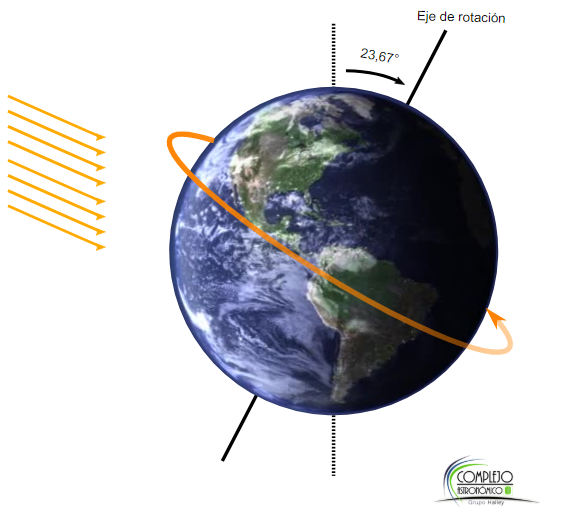
\includegraphics[scale=0.65]{Imagenes/Rotacion_01} 
\caption{Movimiento de Rotación}
\label{m_rotacion}
\end{figure}
La rotación es un movimiento que implica el cambio de orientación de un cuerpo entorno a una línea imaginaria conocida como eje de rotación. En el caso de la Tierra atraviesa el polo sur y norte celeste, y se conoce como eje del mundo. \\

En la antigüedad ``El agua era el inicio, el medio y el fin del cosmo'', esta premisa nace de las culturas antiguas. Las culturas egipcias y babilonias teorizaban sobre el desplazamiento de los astros en la bóveda celeste, concluyendo que estos ``navegaban'' en el cielo como si éste fuera agua que fluye, esto genera una visión geocentrica del cosmos, pues da la impresión de que todo gira en torno a la Tierra. \\

Fueron los primeros filósofos milesios los que cuestionaron estas creencias, como Anaximandro que se preguntó:  ¿Serán los astros del mismo tamaño?, ¿Estarán los astros a la misma distancia de la Tierra? Además de estas preguntas, Anaximandro innovó con el uso del gnomón, instrumento que permitía evidenciar el movimiento aparente del Sol en la bóveda celeste. \\

En la actualidad es posible demostrar, con observaciones desde diferentes puntos geográficos, que la Tierra rota sobre el eje del mundo y que el movimiento aparente de los astros en la bóveda celeste es producto del movimiento de rotación. Un efecto causado por la rotación de la Tierra, sino el más importante, es la existencia del ``día'' y de la ``noche'' junto con la definición de ``un día'', expresión que comprende una rotación completa de la Tierra y que dura aproximadamente 24 horas. \\

Otro de los fenómenos provocados por el movimiento de rotación, es el llamado ``achatamiento de los polo''. El achatamiento se debe a las fuerzas centrífugas que experimente la Tierra al rotar. Al alejarse del centro de rotación (eje de rotación) la fuerza centrífuga es mayor, esto quiere decir que: cuanto más cerca del Ecuador, mayor fuerza centrífuga, y cuanto más lejos (más cerca a los polos), menor es la fuerza centrífuga.

\begin{figure}[H]
\centering
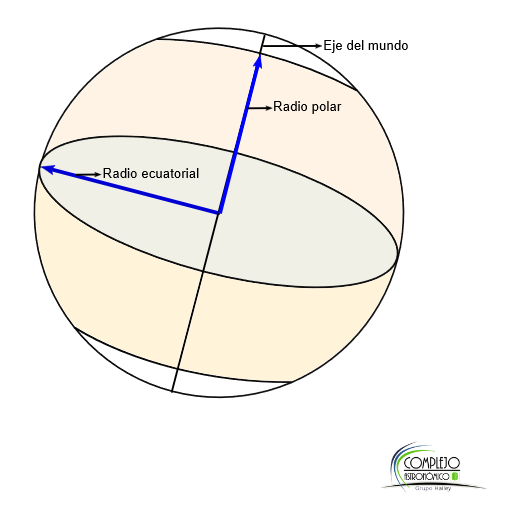
\includegraphics[scale=0.65]{Imagenes/Achatamiento_01} 
\caption{Achatamiento de los polos}
\label{achatamiento}
\end{figure}

\subsection{Traslación}

\begin{figure}[H]
\centering
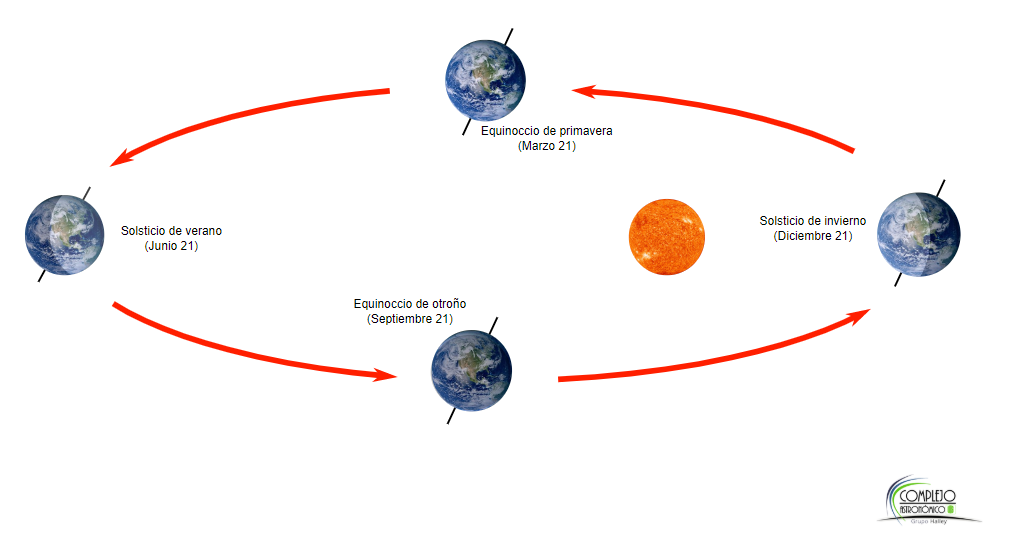
\includegraphics[scale=0.45]{Imagenes/Traslacion_01} 
\caption{Movimiento de Traslación}
\label{m_traslacion}
\end{figure}

Cuando se propuso el movimiento de traslación fue revolucionario. La traslación de la Tierra implicaría una teoría heliocéntrica y acabaría con la geocéntrica, un golpe a las creencias que dominaban épocas oscuras.  \\ 

Debido al movimiento de traslación los cielos cambian en función del tiempo, de esto se derivan historias como la persecución infinita que hace ``el escorpión'' a ``el cazador''. Los antiguos sabían que cuando ``el cazador'' era visible en los cielos, ``el escorpión'' no aparecía, y viceversa. Además, las constelaciones jugaron un papel fundamental en la predicción de sequías y de épocas de lluvia, ayudando en la producción de alimentos cultivados. \\

Aristóteles, aunque promotor de la teoría geocéntrica, observó un fenómeno peculiar en el movimiento aparente de algunos astros, estos erraban del movimientos natural que seguían los otros. Fue así como se les acuñó el nombre de Planetas: errantes que no coinciden con la armonía con la que danzaban los otros astros, otro fenómeno que es explicado con el movimiento de traslación. \\

Los solsticios y equinoccios son dos de los fenómenos más importantes que derivan del movimiento de traslación. En los solsticios el sol alcanza su puntos más alto o más bajo, visto por un observador sobre la Tierra.  Al ser solsticio de verano para el hemisferios sur los rayos solares inciden casi directamente sobre el trópico de Capricornio, y sobre el trópico de Cancer al ser solsticio de verano en el hemisferio norte. En el equinoccio, los rayos solares inciden sobre el paralelo del Ecuador, marcando el inicio de la primavera y el otoño.

\subsection{Precesión}
El movimiento de precesión es el cambio de dirección que experimenta el eje de rotación del planeta Tierra y tiene una duración aproximada de 25800 años, razón por la cual cada 71.6 años la estrella polar se desplaza 1°. 

\begin{figure}[H]
\centering
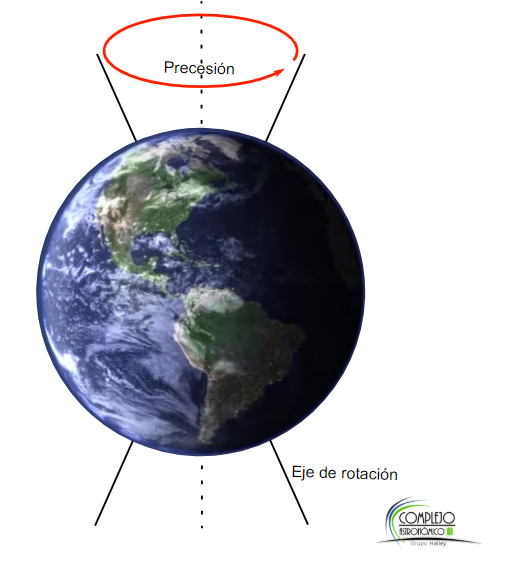
\includegraphics[scale=0.45]{Imagenes/Precesion_01} 
\caption{Movimiento de Precesión}
\label{m_traslacion}
\end{figure}

\subsection{Nutación}
El movimiento de nutación es el causante de que el círculo de la precesión no sea exacto, sino que presenta, en su recorrido, oscilaciones que causan una mayor o menor inclinación del eje de la Tierra. Este movimiento es causado por la influencia gravitatoria de la Luna.

\begin{figure}[H]
\centering
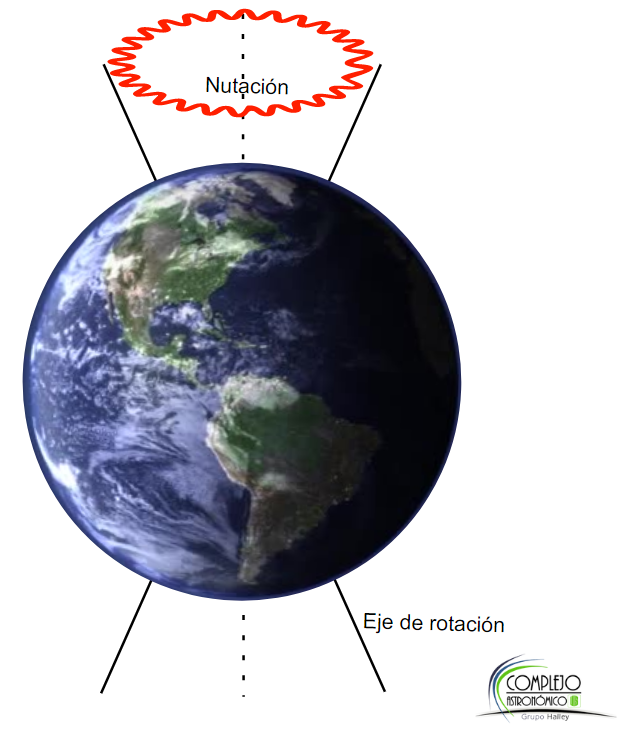
\includegraphics[scale=0.45]{Imagenes/Nutacion_01} 
\caption{Movimiento de Nutación}
\label{m_traslacion}
\end{figure} 

\subsection{Bamboleo de Chandler}
El bamboleo de Chandler es una pequeña variación en el eje de rotación de la Tierra. Consiste en que los polos de la Tierra se mueven en una circunferencia irregular de 3-15 metros de diámetro. Existe poca información consistente sobre las causas de este fenómeno, pero la teoría más prometedora sugiere que; ``la causa principal del bamboleo de Chandler es la presión fluctuante del fondo oceánico, originada por los cambios de temperatura y salinidad, y por los cambios en las direcciones de las corrientes oceánicas ''
\section{Planeación de la sesión}
\begin{table}[h!]
\begin{tabular}{|l|l|l|l|}
\hline
\textbf{Etapa}      & \textbf{Tiempo} & \textbf{Actividad}                                        & \textbf{Recursos}                                                           \\ \hline
\textbf{Inicio}     & 30 minutos      & S02AI01                                                   & \begin{tabular}[c]{@{}l@{}}- Palo de balso \\ - Bisturí \\ - Transportador \\ - Tabla de balso (cartón paja) \\ - Pegamento (silicona)  \end{tabular} \\ \hline
\textbf{Desarrollo} &   60 minutos               & \begin{tabular}[c]{@{}l@{}}S01AD01\\S02AD01\end{tabular} & \begin{tabular}[c]{@{}l@{}}- Proyector\\ - Audio \\
 - Cartulina \\-  Grapadora \\ - Bisturí \\ - Chinches \end{tabular}               \\ \hline
\textbf{Cierre}     &   30 minutos              & S01AC01                                                   & - Tarjetas                                                                  \\ \hline
\end{tabular}
\end{table}

\subsection{S02AI01}
En esta actividad se hará uso de la maqueta que se muestra en la Figura (\ref{maqueta_01}) para evidenciar el movimiento de rotación de la Tierra y su eje de inclinación respecto al plano Eclíptico. Inicialmente se ubicará la maqueta en un lugar abierto y con luz solar; debe apuntar hacia el norte celeste. Luego, se marca el final de la sombra del gnomon de la base; esto se hará cada 5 minutos. Al final se comparará la diferencia en las longitudes de las sombras marcadas y se trazará una linea que una el final de cada marca. Esto evidenciará el movimiento aparente del Sol, asociando este fenómeno con la rotación que presenta la Tierra.

\begin{figure}[H]
\centering
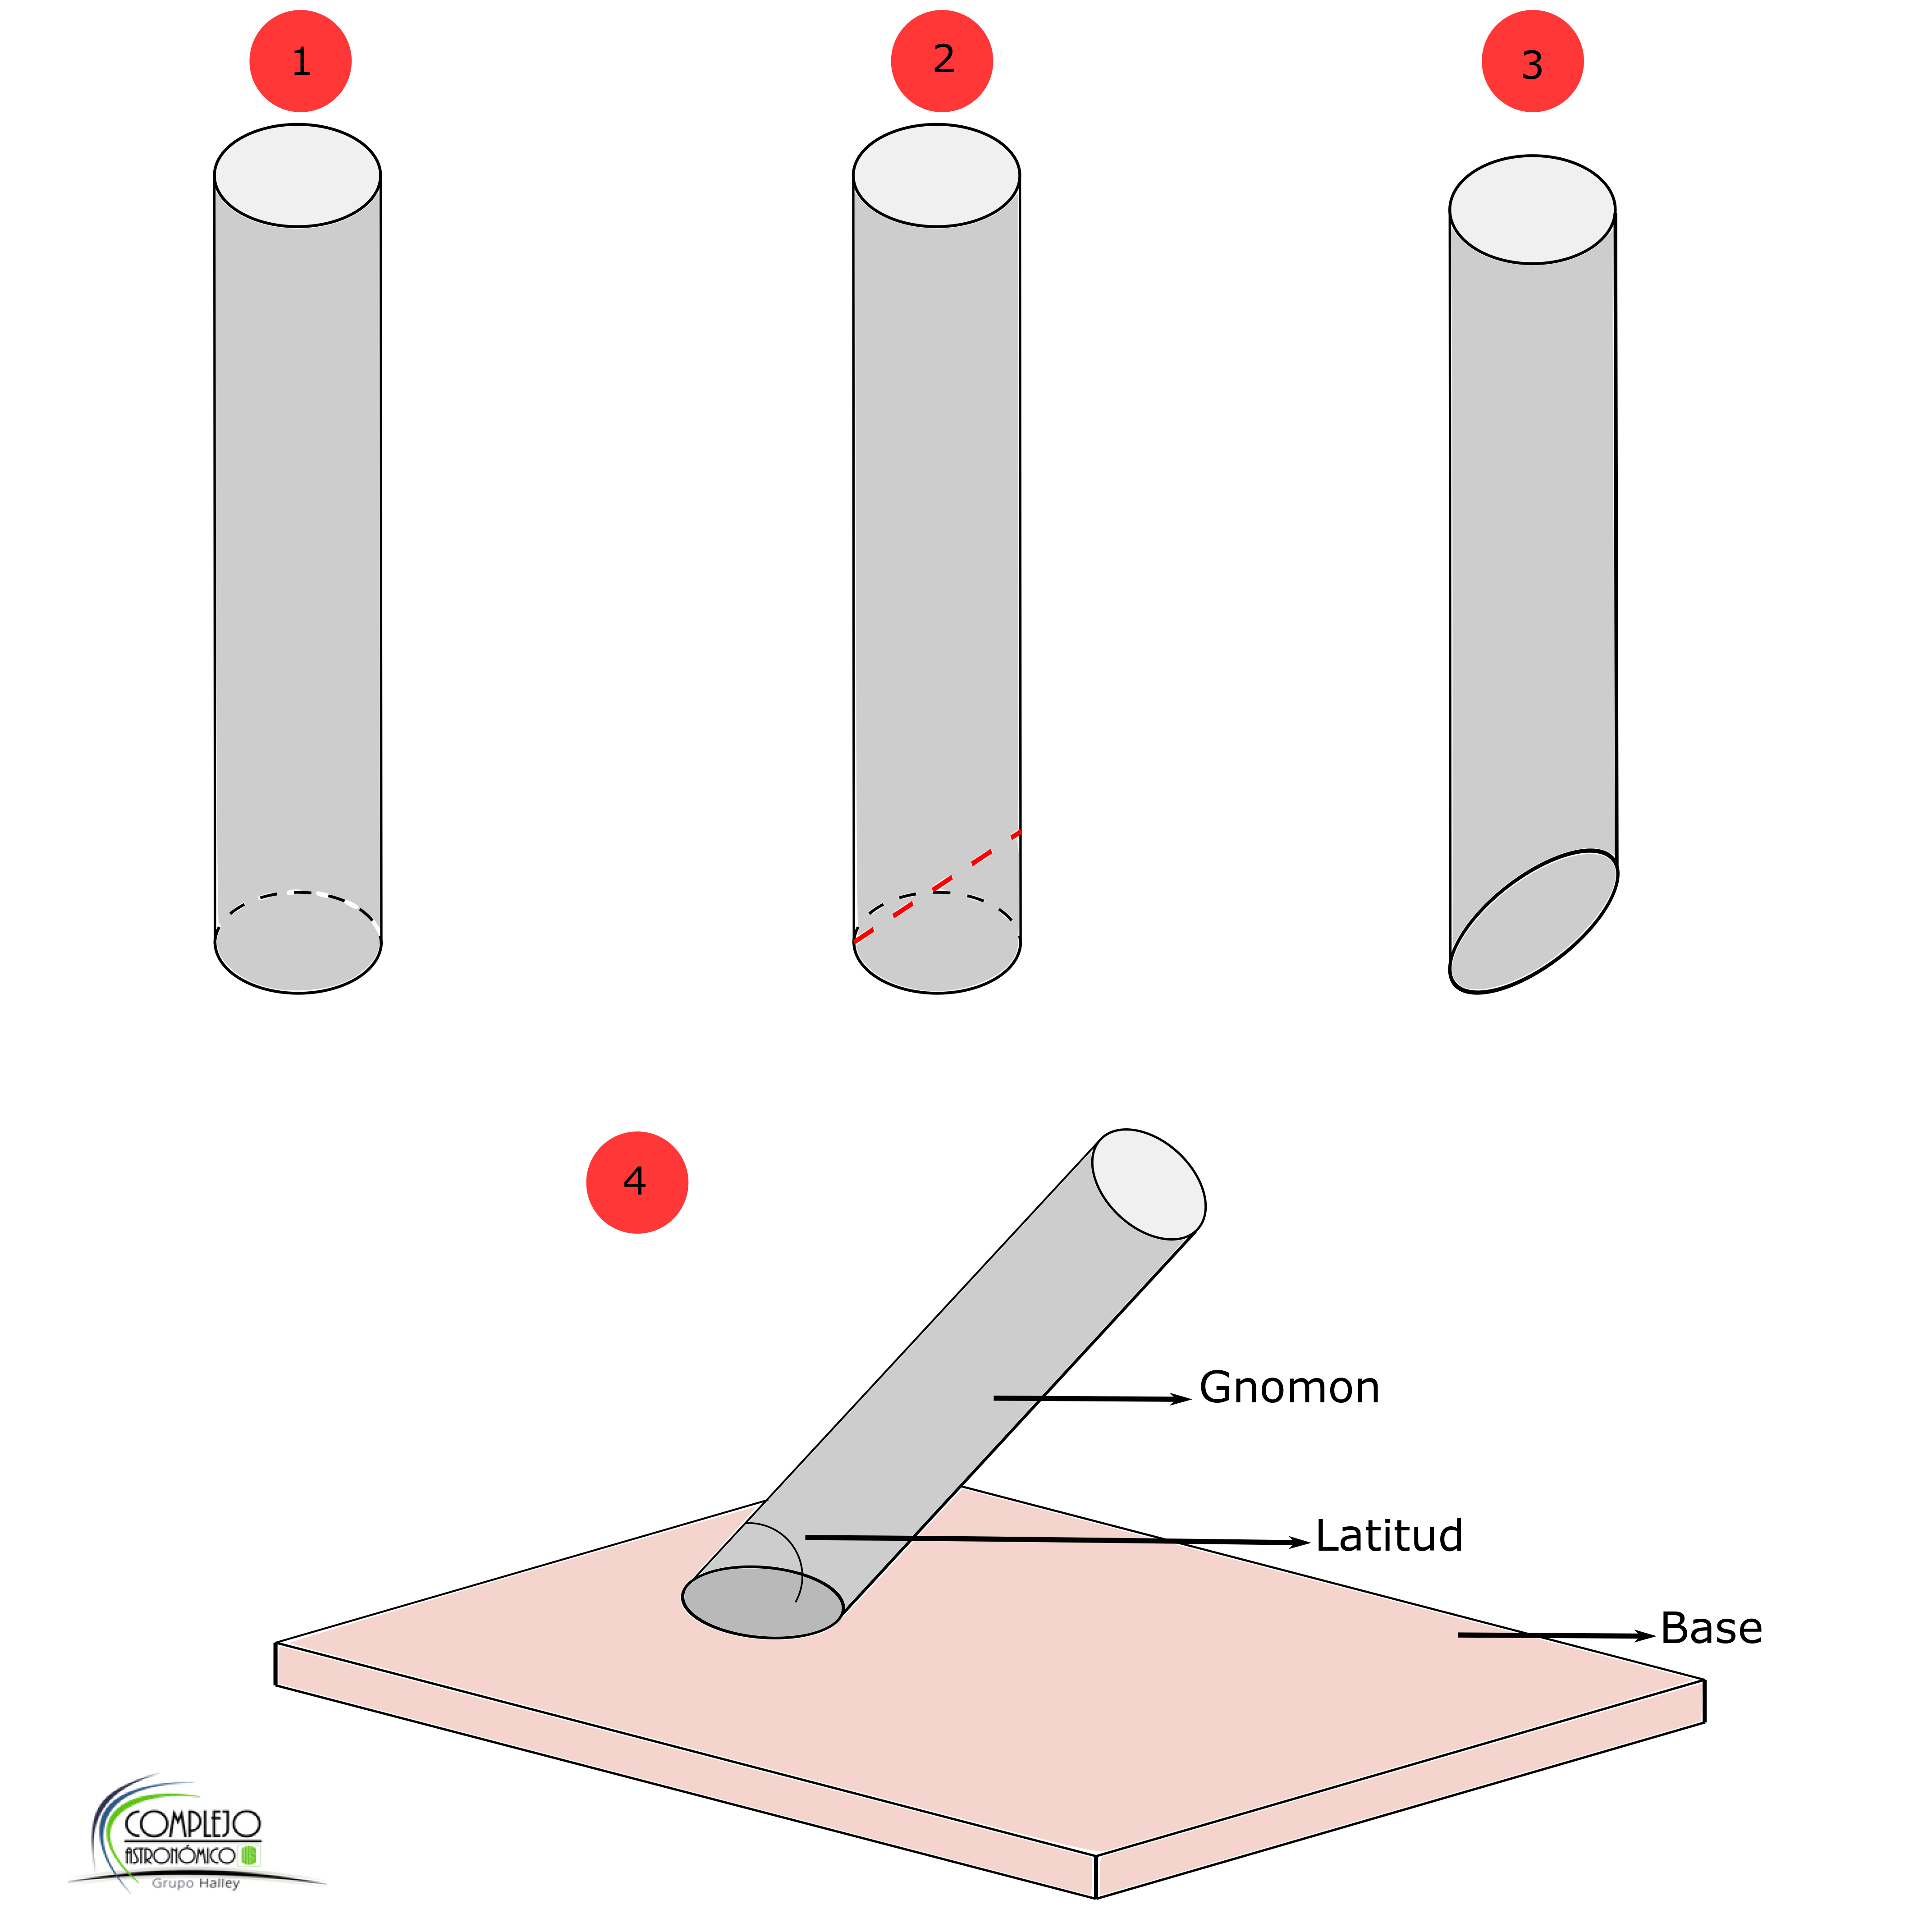
\includegraphics[scale=0.05]{Imagenes/Maqueta_01} 
\caption{Maqueta\_01}
\label{maqueta_01}
\end{figure} 

\subsection{S02AD01}
Para la siguiente actividad se hará uso de la maqueta que se ve en la Figura (\ref{Achatamiento_02}). En esta actividad, cada estudiante fabricará, con ayuda del personal a cargo, una maqueta. En seguida, harán girar el palo de pincho a diferentes velocidades. El propósito es relacionar la velocidad a la que gira el palo de pincho y el cambio de posición de las bandas de papel, de este modo se ejemplifica el achatamiento en los polos de la Tierra.

\begin{figure}[H]
\centering
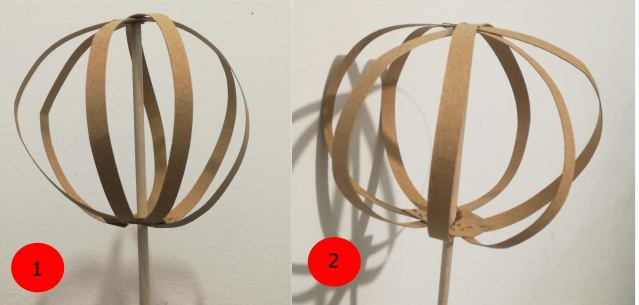
\includegraphics[scale=0.5]{Imagenes/Achatamiento_02.png} 
\caption{Achatamiento de los polos producto de la rotación de la tierra.}
\label{Achatamiento_02}
\end{figure} 


\subsection{S02AD02}


\subsection{S02AC01}
Haciendo uso de la maqueta \textbf{name} se sintetizará los movimientos antes expuestos. Con la maqueta es posible evidenciar el movimiento de traslación y cómo este junto a la inclinación del eje del mundo  da origen a los solsticios y equinoccios, lo que marca el cambio de las estaciones. También, al existir un ``eje del mundo'' visible en la maqueta, se puede evidenciar el cambio en la dirección del mismo, este fenómeno es causado por los movimientos de: precesión, nutación y bamboleo de Chandler.
\end{document}
